%%%%%%%%%%%%%%%%%%%%%%%%%%%%%%%%%%%%%%%%%
% Compact Laboratory Book
% LaTeX Template
% Version 1.0 (4/6/12)
%
% This template has been downloaded from:
% http://www.LaTeXTemplates.com
%
% Original author:
% Joan Queralt Gil (http://phobos.xtec.cat/jqueralt) using the labbook class by
% Frank Kuster (http://www.ctan.org/tex-archive/macros/latex/contrib/labbook/)
%
% License:
% CC BY-NC-SA 3.0 (http://creativecommons.org/licenses/by-nc-sa/3.0/)
%
% Important note:
% This template requires the labbook.cls file to be in the same directory as the
% .tex file. The labbook.cls file provides the necessary structure to create the
% lab book.
%
% The \lipsum[#] commands throughout this template generate dummy text
% to fill the template out. These commands should all be removed when 
% writing lab book content.
%
% HOW TO USE THIS TEMPLATE 
% Each day in the lab consists of three main things:
%
% 1. LABDAY: The first thing to put is the \labday{} command with a date in 
% curly brackets, this will make a new section showing that you are working
% on a new day.
%
% 2. EXPERIMENT/SUBEXPERIMENT: Next you need to specify what 
% experiment(s) and subexperiment(s) you are working on with a 
% \experiment{} and \subexperiment{} commands with the experiment 
% shorthand in the curly brackets. The experiment shorthand is defined in the 
% 'DEFINITION OF EXPERIMENTS' section below, this means you can 
% say \experiment{pcr} and the actual text written to the PDF will be what 
% you set the 'pcr' experiment to be. If the experiment is a one off, you can 
% just write it in the bracket without creating a shorthand. Note: if you don't 
% want to have an experiment, just leave this out and it won't be printed.
%
% 3. CONTENT: Following the experiment is the content, i.e. what progress 
% you made on the experiment that day.
%
%%%%%%%%%%%%%%%%%%%%%%%%%%%%%%%%%%%%%%%%%

%----------------------------------------------------------------------------------------
%	PACKAGES AND OTHER DOCUMENT CONFIGURATIONS
%----------------------------------------------------------------------------------------                               

\documentclass[fontsize=11pt, % Document font size
                             paper=a4, % Document paper type
                             twoside, % Shifts odd pages to the left for easier reading when printed, can be changed to oneside
                             captions=tableheading,
                             index=totoc,
                             hyperref]{labbook}
 
\usepackage[bottom=10em]{geometry} % Reduces the whitespace at the bottom of the page so more text can fit

\usepackage[english]{babel} % English language
\usepackage{lipsum} % Used for inserting dummy 'Lorem ipsum' text into the template

\usepackage[utf8]{inputenc} % Uses the utf8 input encoding
\usepackage[T1]{fontenc} % Use 8-bit encoding that has 256 glyphs

\usepackage[osf]{mathpazo} % Palatino as the main font
\linespread{1.05}\selectfont % Palatino needs some extra spacing, here 5% extra
\usepackage[scaled=.88]{beramono} % Bera-Monospace
\usepackage[scaled=.86]{berasans} % Bera Sans-Serif

\usepackage{booktabs,array} % Packages for tables

\usepackage{amsmath} % For typesetting math
\usepackage{graphicx} % Required for including images
\usepackage{etoolbox}
\usepackage{fancyvrb}
\usepackage{float}
\usepackage[norule]{footmisc} % Removes the horizontal rule from footnotes
\usepackage{lastpage} % Counts the number of pages of the document

\usepackage[dvipsnames]{xcolor}  % Allows the definition of hex colors
\definecolor{titleblue}{rgb}{0.16,0.24,0.64} % Custom color for the title on the title page
\definecolor{linkcolor}{rgb}{0,0,0.42} % Custom color for links - dark blue at the moment

\addtokomafont{title}{\Huge\color{titleblue}} % Titles in custom blue color
\addtokomafont{chapter}{\color{OliveGreen}} % Lab dates in olive green
\addtokomafont{section}{\color{Sepia}} % Sections in sepia
\addtokomafont{pagehead}{\normalfont\sffamily\color{gray}} % Header text in gray and sans serif
\addtokomafont{caption}{\footnotesize\itshape} % Small italic font size for captions
\addtokomafont{captionlabel}{\upshape\bfseries} % Bold for caption labels
\addtokomafont{descriptionlabel}{\rmfamily}
\setcapwidth[r]{10cm} % Right align caption text
\setkomafont{footnote}{\sffamily} % Footnotes in sans serif

\deffootnote[4cm]{4cm}{1em}{\textsuperscript{\thefootnotemark}} % Indent footnotes to line up with text

\DeclareFixedFont{\textcap}{T1}{phv}{bx}{n}{1.5cm} % Font for main title: Helvetica 1.5 cm
\DeclareFixedFont{\textaut}{T1}{phv}{bx}{n}{0.8cm} % Font for author name: Helvetica 0.8 cm

\usepackage[nouppercase,headsepline]{scrpage2} % Provides headers and footers configuration
\pagestyle{scrheadings} % Print the headers and footers on all pages
\clearscrheadfoot % Clean old definitions if they exist

\automark[chapter]{chapter}
\ohead{\headmark} % Prints outer header

\setlength{\headheight}{25pt} % Makes the header take up a bit of extra space for aesthetics
\setheadsepline{.4pt} % Creates a thin rule under the header
\addtokomafont{headsepline}{\color{lightgray}} % Colors the rule under the header light gray

\ofoot[\normalfont\normalcolor{\thepage\ |\  \pageref{LastPage}}]{\normalfont\normalcolor{\thepage\ |\  \pageref{LastPage}}} % Creates an outer footer of: "current page | total pages"

% These lines make it so each new lab day directly follows the previous one i.e. does not start on a new page - comment them out to separate lab days on new pages
\makeatletter
\patchcmd{\addchap}{\if@openright\cleardoublepage\else\clearpage\fi}{\par}{}{}
\makeatother
\renewcommand*{\chapterpagestyle}{scrheadings}

% These lines make it so every figure and equation in the document is numbered consecutively rather than restarting at 1 for each lab day - comment them out to remove this behavior
\usepackage{chngcntr}
\counterwithout{figure}{labday}
\counterwithout{equation}{labday}

% Hyperlink configuration
\usepackage[
    pdfauthor={}, % Your name for the author field in the PDF
    pdftitle={Cleaning and Mapping Robot Laboratory Journal}, % PDF title
    pdfsubject={}, % PDF subject
    bookmarksopen=true,
    linktocpage=true,
    urlcolor=linkcolor, % Color of URLs
    citecolor=linkcolor, % Color of citations
    linkcolor=linkcolor, % Color of links to other pages/figures
    backref=page,
    pdfpagelabels=true,
    plainpages=false,
    colorlinks=true, % Turn off all coloring by changing this to false
    bookmarks=true,
    pdfview=FitB]{hyperref}

\usepackage[stretch=10]{microtype} % Slightly tweak font spacing for aesthetics

%\setlength\parindent{0pt} % Uncomment to remove all indentation from paragraphs

%----------------------------------------------------------------------------------------
%	DEFINITION OF EXPERIMENTS
%----------------------------------------------------------------------------------------

% Template: \newexperiment{<abbrev>}[<short form>]{<long form>}
% <abbrev> is the reference to use later in the .tex file in \experiment{}, the <short form> is only used in the table of contents and running title - it is optional, <long form> is what is printed in the lab book itself

\newexperiment{example}[Example experiment]{This is an example experiment}
\newexperiment{example2}[Example experiment 2]{This is another example experiment}
\newexperiment{example3}[Example experiment 3]{This is yet another example experiment}

\newsubexperiment{subexp_example}[Example sub-experiment]{This is an example sub-experiment}
\newsubexperiment{subexp_example2}[Example sub-experiment 2]{This is another example sub-experiment}
\newsubexperiment{subexp_example3}[Example sub-experiment 3]{This is yet another example sub-experiment}

%----------------------------------------------------------------------------------------

\begin{document}

%----------------------------------------------------------------------------------------
%	TITLE PAGE
%----------------------------------------------------------------------------------------

\title{\textcap{Cleaning and Mapping Robot Laboratory Journal \\[1cm]  
\textaut{Beginning 5-27-2020}}}

\author{
    \textaut{Brian Lauer}\\ \\ % Your name
}
\date{} % No date by default, add \today if you wish to include the publication date

\maketitle % Title page

\printindex
\tableofcontents % Table of contents
\newpage % Start lab look on a new page

\begin{addmargin}[0cm]{0cm} % Makes the text width much shorter for a compact look

\pagestyle{scrheadings} % Begin using headers

%----------------------------------------------------------------------------------------
%	LAB BOOK CONTENTS
%----------------------------------------------------------------------------------------

\labday{Wednesday, May 27, 2020}
Problem Statement:\\
Various cleaning and mapping (CAM) robots such as the Roomba by iRobot are commercially available today and are able to clean different areas of a home or business. Some of the top of the line robots by iRobot like the Roomba s9+, Roomba i7+, and Braava m6 are able to map rooms with a technology called Imprint Smart Mapping technology. In the app for each robot, a clean map report can be generated\footnote{\url{https://homesupport.irobot.com/app/answers/detail/a_id/1467}}. The generated 2D map will show areas that were cleaned by the robot and the white areas that contained obstacles like furniture or appliances. In these robots that support the mapping feature, a camera is mounted at an angle of 45 degrees that takes pictures of a room regularly. These images are then processed using Visual Simultaneous Localization and Mapping (VSLAM)\footnote{\url{https://www.thezebra.com/resources/home/how-roomba-works/}}. Multiple alternative techniques for localization and mapping a robot including lidar and RFID technology. In the proposed research, RFID technology will be utilized for the purpose of possibly lowering costs and computational complexity.
\smallbreak\noindent
Research efforts:\\
In~\cite{hahnel2004}, a probabilistic model for localizing an RFID tag is given for the purpose of localizing a robot in its environment. Given a the position $x$ of the tag and data $z_{1:t}$, the probability of obtaining the correct position of the robot given the observations is 
\[
p(x|z_{1:t})=\alpha p(z_t \vert x) p(x \vert z_{1:t-1})
\]
where $\alpha$ is the normalization constant. The purpose of this study was to determine the locations of RFID tags in an office building using a laser range finder and an RFID reader mounted on the robot. With the RFID tag's locations the path of the robot could be estimated which is known as localization. However, it does not use RFID specifically for mapping an environment. Therefore, techniques must be found for determining how to map the robot's environment. This may only be possible with sensors like a laser range finder, LIDAR sensor, or other digital devices like a camera.

\labday{Thursday, May 28, 2020}
I received the resources for the iRobot Create 2 from Jaden today in his Google Drive. The iRobot Create 2 is a hackable device designed for education rather than commercial use\footnote{\url{https://www.irobot.com/About-iRobot/STEM/Create-2/Projects.aspx}}. On iRobot's site, many different projects have been done with this robot such as a Nerf-gun mounted turret modification, nerf-gun dart collector robot, camera bot, pokemon go egg hatching, zcm driver, and path finder. All of them are documented in the provided footnote.

\labday{Monday, June 1, 2020}
Today, I did some research on how to implement the mapping feature with a LIDAR sensor as Prof. Miah mentioned that this technology is available in some of the labs. I looked at a tutorial on how to interface the Neato LIDAR sensor with a Beaglebone~\footnote{\url{https://www.alexschimp.com/neato-lidar-data-beaglebone-black/}}. By simply connecting the LIDAR sensor to the TX and RX pins of the board, data can be sent to the device or the encoded can be retrieved. The mentioned LIDAR comes with a motor which can be powered with a $3$V power supply. To read from the device the device file in the \texttt{/dev} directory must be opened. Each packet consists of 22 bytes. The code below:
\begin{Verbatim}
print("Hello")

with open("/dev/ttyO2", "rb") as f:
    byte = f.read(1)
    count = 1
    while byte != "" and count <= 22*100:
        print(byte.encode('hex') + ":")
        byte = f.read(1)
        count += 1

print("Goodbye")
\end{Verbatim}
where the LIDAR is located at \texttt{/dev/tty02}. However, the LIDAR sensor that Prof. Miah has in his robotics lab is likely different as there are a lot of different options out there.

\labday{Tuesday, June 2, 2020}
In yesterday's meeting with Jaden, my partner, we agreed that he would focus mostly on the hardware side of things as he has the robot and beaglebone while I work on building an Android app for showing the map. In this way, I will be able to make more of a significant contribution toward the project with the resources I currently have. I have never built an app before so some research will be required before I start developing the app.
\smallbreak\noindent
I started by following the Android tutorial\footnote{\url{https://developer.android.com/training/basics/firstapp/creating-project}}. The UI for each app is built using a system of layouts and widgets where the layouts are \texttt{ViewGroup} objects and the widgets are \texttt{View} objects. Objects in the layout like text objects and buttons can be constrained to each other. For each TextView object, a \texttt{textSize} and \texttt{textColor} variable can be set. The result of the tutorial is shown below:
\begin{figure}[H]
\centering
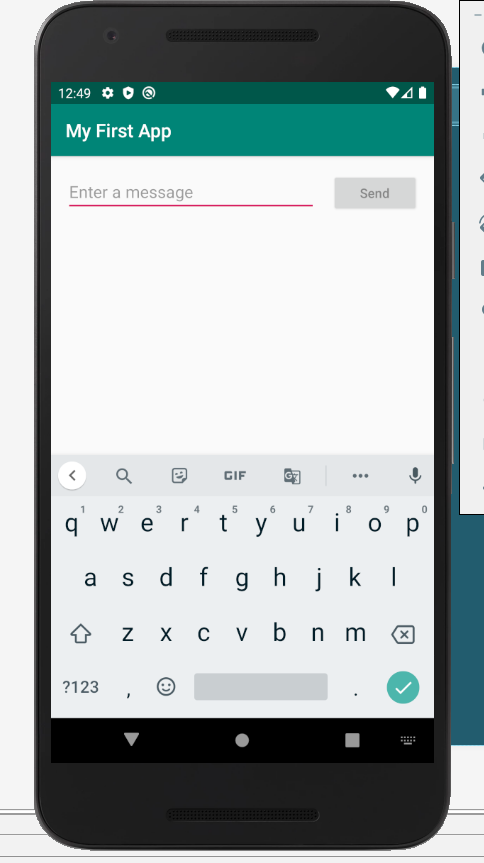
\includegraphics[scale=0.5]{figs/img/myFirstApp}
\end{figure}
where after text is entered and the button is pressed, a new activity is shown which displays the text under the top app bar.

\labday{Wednesday, June 3, 2020}
Today I took a pause on developing the app by looking at the link to the Lidar sensor that Dr. Miah sent us that is available in the robotics facility~\footnote{\url{https://www.robotshop.com/en/rplidar-s1-360-laser-scanner-40-m.html?utm_source=google&utm_medium=surfaces&utm_campaign=surfaces_across_google_usen&gclid=EAIaIQobChMI9JyBto7m6QIVkIbACh3GMwhZEAYYASABEgIebPD_BwE}}. 
The model is a RPiLIDAR S$1$ $360^\circ$. According to the datasheet it can perform 2D $360^\circ$ scan of an area with a 40 meter range. The sampling rate is 9200 samples per second and the sensor can tilt vertically up $0.391^\circ$. While scanning, the data output of the sensor over UART includes both the distance between the rotating LIDAR sensor and the sampling point while the heading is the current angle of measurement in degrees. A flag in the data will signal the start of a new scan. Both the distance and heading values will be sent as pairs for data communication for each sample point. The pinout for the device is as follows:

\begin{center}
\begin{tabular}{|c|c|}
\hline
Pin Name & Description \\
VCC & Power\\
GND & Power\\
RX & Serial Input\\
TX & Serial Output\\
\hline
\end{tabular}
\end{center}
where there are two pins for VCC and GND each as separate power is needed for the sensor and motor system that rotates the sensor. Because the connector used for the sensor is a SH$1.0$-$6$P, some special wires may be needed for connecting to the device. As far as the specification for the serial interface goes, the baud rate is 256000 bps and uses 3.3V TTL logic.
\smallbreak\noindent
Since I am on my laptop and do not have android studio installed on it, I began installing it. I realized that the Create 2 does not have any sort of internet connectivity, so a web server will be needed on the Beaglebone to communicate with it wirelessly. In the app, some functionality will need to be developed to discover the Roomba on the network. 
\smallbreak\noindent
I created a new project called LidarMap using the bottom navigation bar template.

\labday{Thursday, June 4, 2020}
I spent some time wireframing the UI for the app on paper today. The app will have a bottom navigation bar with the pages Discovery and Map. The Discovery page will contain the list of discovered robots while the Map page will contain the map similar to the map shown in the Roomba app. Similar to my building energy management project, the robots should be discovered automatically with an "autodiscovery" feature. While waiting for devices to be discovered I want to add an indefinite progress bar spinner. Since I realized that it is possibly going to be more difficult to change the current icons in the current app I decided that I will simply start making the app using a blank template.
\smallbreak\noindent
I thus created a new Android Studio project named \texttt{Create2LidarMap} using Android 4.0.3 (Ice Cream Sandwich) using the empty activity template. I then followed~\footnote{\url{https://androidwave.com/bottom-navigation-bar-android-example/}} to create a bottom nav bar from scratch. 

\labday{Friday, June 5, 2020}
I worked on adding the bottom navigation menu from scratch into the app. The icons were successfully added where one is a magnifying glass and the other is a quilt for the map page. The \texttt{NavHostFragment} component in the MainAcitity page will provide an area above the nav menu for self contained navigation to occur. Essentially two different fragments will be created for the discovery and map respectively. However after adding the component to the main activity and importing the Android jetpack package \texttt{androidx.navigation.fragment}, I got a warning stating that to Replace the tag With FragmentContainerView. I made the change to this View but another issue came up as the navGraph attribute excepts a resource of type String but currently has a navigation resource type (@navigation/mobile\_navigation). Inside the onCreate method in the \texttt{MainActivity} class, I added the line
\begin{Verbatim}
this.getSupportActionBar().hide();
\end{Verbatim}
To remove the top action bar with the name of the activity which in my opinion makes the app look a little cleaner.

\labday{Monday, June 8, 2020}
Because of the issues mentioned previously with adding the navbar from a blank project, I decided to simply take the original LidarMap project and modify it with the appropriate fragment and subtract and add the appropriate navbar elements. In the java directory I created a package\texttt{com.example.ui.lidarmap.map} where I created the java file \texttt{MapFragment.java} and \texttt{MapViewModel.java}. The source code for MapFragment was generated by default and contains the following:
\begin{Verbatim}
package com.example.lidarmap.ui.map;

import androidx.lifecycle.ViewModelProviders;

import android.os.Bundle;

import androidx.annotation.NonNull;
import androidx.annotation.Nullable;
import androidx.fragment.app.Fragment;

import android.view.LayoutInflater;
import android.view.View;
import android.view.ViewGroup;

import com.example.lidarmap.R;

public class MapFragment extends Fragment {

    private MapViewModel mViewModel;

    public static MapFragment newInstance() {
        return new MapFragment();
    }

    @Override
    public View onCreateView(@NonNull LayoutInflater inflater, 
    @Nullable ViewGroup container,
                             
                            @Nullable Bundle savedInstanceState) {
        return inflater.inflate(R.layout.map_fragment, container, false);
    }

    @Override
    public void onActivityCreated(@Nullable Bundle savedInstanceState) {
        super.onActivityCreated(savedInstanceState);
        mViewModel = ViewModelProviders.of(this).get(MapViewModel.class);
        // TODO: Use the ViewModel
    }

}
\end{Verbatim}
I created a second package named \texttt{com.example.lidarmap.ui.discovery} with the files \texttt{DiscoveryFragment} and \texttt{DiscoveryViewModel} which similar code to the map fragment and view model classes. After adding these files, I generated the layout files. However, the build failed with the exception: \texttt{java.lang.RuntimeException}. I thus decided to once again create a new project from scratch in hopes of fixing the previous issues from the \texttt{CAMRobotMap} project.
\smallbreak\noindent
I decided to scrap all my previous ideas and simply follow a tutorial on Youtube at \footnote{\url{https://www.youtube.com/watch?v=tPV8xA7m-iw}}. At the beginning of the tutorial, the speaker mentioned that if only two destinations are needed (map, discovery) then it is better to use a tab layout instead. I deleted the old project with the bottom nav and created a new project with tabbed activity template. Instead I decided the follow the tutorial \footnote{\url{https://www.youtube.com/watch?v=h4HwU_ENXYM}}. In the "Discovery" tab, I added a ListView object 

\labday{Wednesday, June 10, 2020}
What I plan on accomplishing today is creating a github repository for the android app and sharing with Jaden, so that we can both work on the software together as he cannot do much due to hardware limitations with the Roomba. Next I would like to start writing a method to create a TCP/UDP client and send out broadcast messages on the network for the Roomba. First, I asked Dr. Miah for permission before pushing the project to a public Github repository. However, I found that I recent change was made to github that allows for unlimited private repos with fewer than 3 or 4 collaborators. When attempting to the push the changes to the repository I got the error:
\begin{verbatim}
Push rejected: Push to origin/master was rejected
\end{verbatim}
This was fixed after I rebased from master to refs/remotes/origin/master. Thus, I was able to succesfully push the project to the github repo LidarMappingRobot.
\smallbreak\noindent
Although the priority is to write the TCP/IP client code for the app, I would like to add subitems into the list view for the Discovery fragment. 

\labday{Thursday, June 11, 2020}
\begin{figure}[H]
\centering
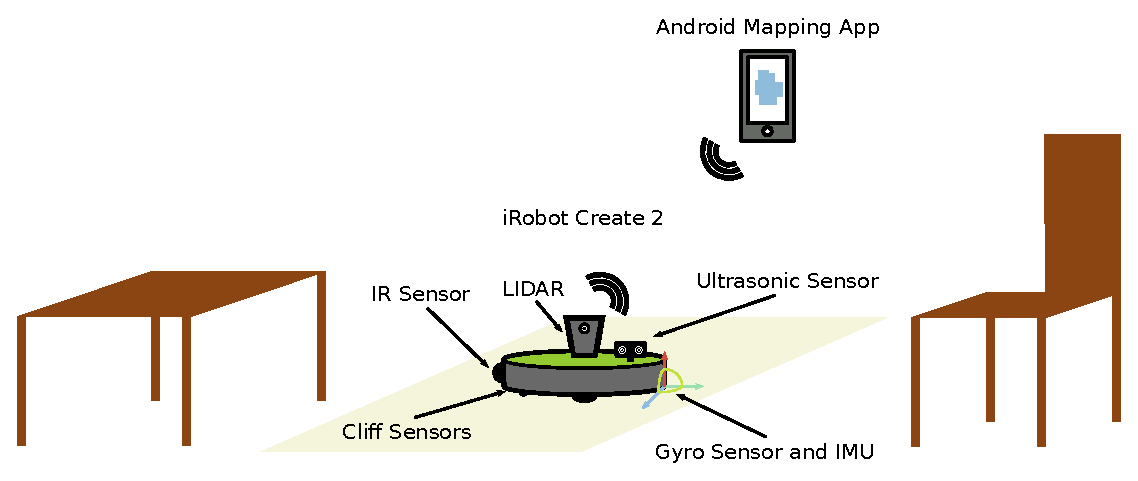
\includegraphics[scale=0.7]{figs/inkscape/mappingRobotArchitecture.eps}
\caption{Diagram representing the working principal of the cleaning and mapping robot}
\end{figure}
\noindent
Description:
\smallbreak
The proposed cleaning and mapping robot based off the Roomba vacuum by iRobot will have the ability to collect sensor data from multiple onboard sensors connected to a single board computer (Beaglebone Blue) for the purpose of localization and mapping. IR sensors, ultrasonic sensors, cliff sensors, and LIDAR will help the robot to understand its environment better. The IMU and gyroscope will help to track orientation, velocity, and rotation. With the aid of the computer, the robot will be able to successfully map its environment like a floor of a house or building. The LIDAR sensor will perform a continuous $360^\circ$ sweep of the environment to generate a $2$D map of the environment. For visualizing the fully completed map, an Android app will be developed to display the outcome of the mapping graphically. Built-in WiFi support of the Beaglebone will act as the communication medium between the robot and client. iRobot has developed a technology of their own that can perform mapping of an area and identify areas of high dirt or dust concentration. However, the robot to be developed will seek to use cost effective sensors to clean the floor and build a map of the environment. The robot will exhibit human like reasoning and intelligence including perception and memory through storage of maps on the single board computer. Techniques like artificial intelligence will be deployed for improving the human like perception abilities of the device even further. 
\end{addmargin}

%----------------------------------------------------------------------------------------
%	BIBLIOGRAPHY
%----------------------------------------------------------------------------------------

\bibliography{bib/cam.bib}
\bibliographystyle{plain}
%----------------------------------------------------------------------------------------

\end{document}